\subsubsection{Repositorios}
Ahora, en las figuras \ref{fig:DR1} y \ref{fig:DR2}, se mostrará más a detalle las propiedades y los métodos de cada una de las clases de tipo repositorio que se encuentran dentro del servidor.

\begin{figure}[htbp!]
	\begin{center}
		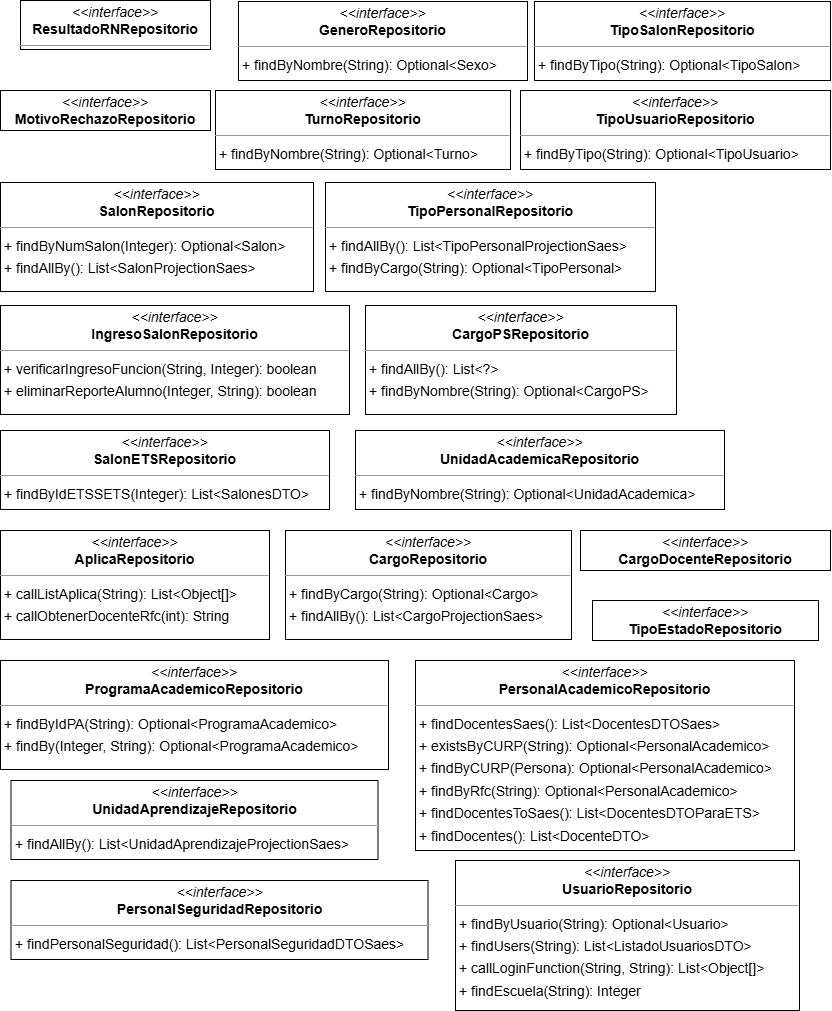
\includegraphics[width=0.8\textwidth]{Clases/Repo1.png}
		\caption{Diagrama de clases de los repositorios del servidor parte 1.}
		\label{fig:DR1}
	\end{center}
\end{figure}

\begin{figure}[htbp!]
	\begin{center}
		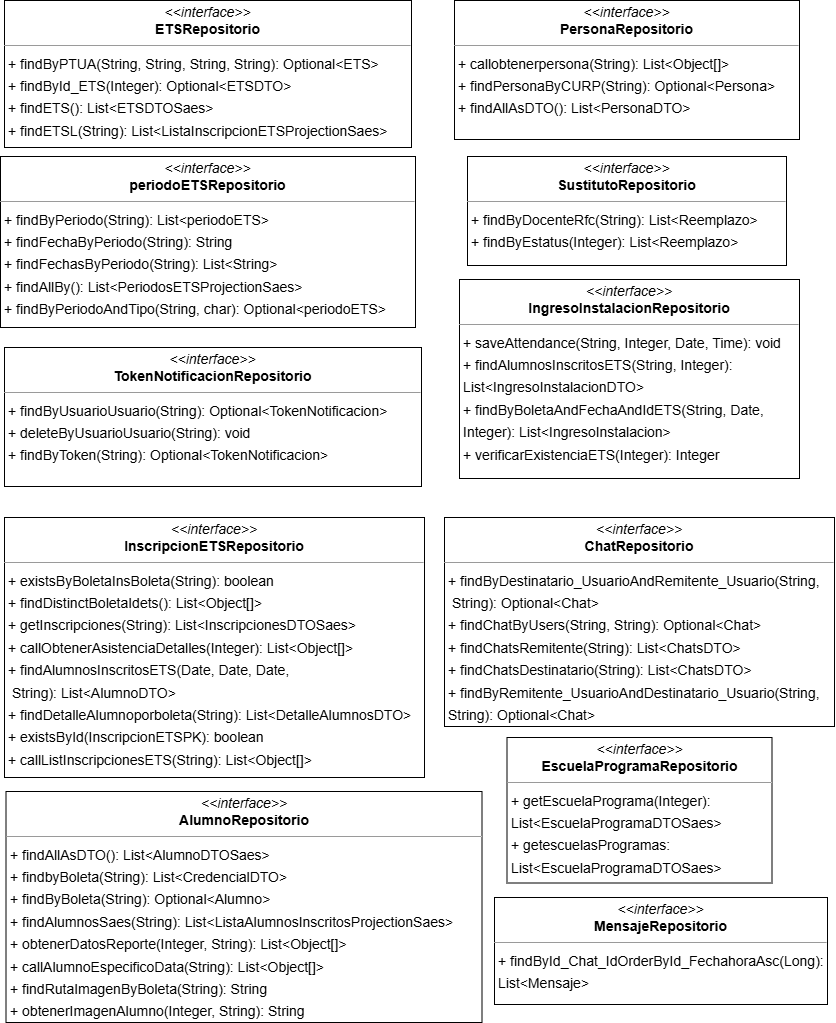
\includegraphics[width=0.8\textwidth]{Clases/Repo2.png}
		\caption{Diagrama de clases de los repositorios del servidor parte 2.}
		\label{fig:DR2}
	\end{center}
\end{figure}